\documentclass[12pt]{article}
\usepackage{mathpazo}
\usepackage{graphicx}
\usepackage[explicit]{titlesec}
\usepackage{hyperref}
\usepackage{xcolor}
\usepackage[export]{adjustbox}
\usepackage{placeins}
\graphicspath {{Images/}}
\hypersetup{
    colorlinks=true,
    linkcolor=black,
    filecolor=magenta,      
    urlcolor=darkgray
}


	\titleformat{\section}[display]
  {\normalfont\scshape\Huge}
  {\hspace*{-70pt}\thesection.~#1}
  {-15pt}
  {\hspace*{-110pt}\rule{\dimexpr\textwidth+80pt\relax}{3pt}\Huge}

\titleformat{name=\section,numberless}[display]
  {\normalfont\scshape\Huge}
  {\hspace*{-70pt}#1}
  {-15pt}
  {\hspace*{-110pt}\rule{\dimexpr\textwidth+80pt\relax}{3pt}\Huge}
\titlespacing*{\section}{0pt}{0pt}{30pt}	


\begin{document}
		 
	 \begin{center}
 	 	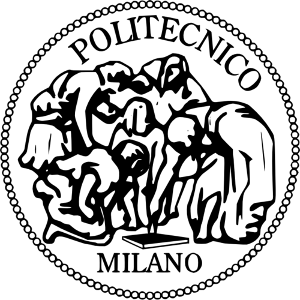
\includegraphics[scale=1.5]{Images/PolimiLogo.png}
	 \end{center}

	 \begin{center}
	 	{\Huge Politecnico di Milano}\\
	 	\vspace{5mm}
		{\Large A.A 2016-2017} 
		\vspace{5mm}\\
		{\huge Requirements Analysis and Specifications Document}   
		\vspace{5mm}\\
		{\large Version 1.0}  
     \end{center}
     
     \begin{center}
		\noindent\rule{8cm}{0.8pt}
		 \vspace{5mm}\\
 	 	 
\includegraphics[scale=1]{Images/logoPowerEnjoy2.png}\\
		\noindent\rule{8cm}{0.8pt}
	 \end{center}
	 	\vspace{5mm}
	
	 \begin{center}
	 	{\Large Instructor : Prof. Di Nitto}
	 	\vspace{5mm}\\	 
	 	{\Large Authors:}\\
	 	{\Large Amico Simone}\\
	 	{\Large Chianella Claudia Beatrice}\\
	 	{\Large Giovanakis Yannick}
	 \end{center}
	 
	 \newpage
	 
	 \tableofcontents{}
	 
	 \newpage
	 
	 \section{\Large Introduction}
	 
	 \subsection{Purpose}
		The aim of this document	is to give an overview of the 	requirements and specifications of system to be developed. 
		The goal of the document is to describe in detail all functional and non-functional requirements of the system, analyzing the needs of the customer and explaining common use case scenarios.
		It will set a baseline for project planning and cost estimation, giving a detailed insight to all stakeholders which include the PowerEnjoy Board , Investors and finally engineers (present and future) involved  in development, testing and maintenance.
		
	 
	 \subsection{System}
	 The to be developed software system provides a complete support to the new PowerEnjoy car-sharing service. It will allow users to register ,log-in and use the car sharing service within the limits imposed by the below specifications.
	 
	
	 
	 \subsection{\label{scope:1}Scope}
	The new PowerEnjoy software system will allow visitors to register and retrieve all necessary information of common domain ( ToS , contact information...). \\Once the visitor has successfully registered to the system and his/her driving license has been approved, he/she will be provided with a unique username-password combination. This enables an user to log into the system at any time , from any mobile device. \\Once logged in, the user can search within a certain distance for vehicles based on his/her current location or based on an input address. 
	Eventually the user chooses to reserve an available vehicle, which can be picked-up within a time span of one hour.\\ 
	Should the user not pick-up the car within the one hour availability limit, then the system will tag the vehicle as available and charge the user a fee of 1 Euro.\\
	Should the user reach the car within the limit,he/she must be able to  interact with the system in order to unlock the vehicle and grant the user access to the car.
	As soon as the engine ignites,the system starts charging the user for a given amount of money per minute. The current charge will be notified through a display inside the car.\\
	The system stops charging the user as soon as the car is parked in a safe area and the user exits the car. At this point the system will automatically lock the car.
	Should the user stop in a non-safe area he/she won't be granted to end the transaction and will be charged until  he/she parks in a safe area.
	The set of safe area parking spots is defined inside the system and must be available all the time to the user's knowledge through the on-board display.
	
	\subsubsection{Goals}
	The PowerEnjoy software system needs to be:
	\begin{itemize}
		\item \textbf{[G1] : Practical}\\It wants to give the users a better connectivity among places in the participant cities that common public transport often can't offer.
		\item \textbf{[G2] : Convenient}\\The service needs to be convenient: it's less expensive than taking a taxi. It's an eco-friendly solution : car-sharing reduces the number of vehicles circulating in the cities and doesn't pollute thanks to electric engines.
		\item \textbf{[G3] : User friendly}\\ The system needs to be as user friendly as possible in order to be used easily by everyone through their own intuitive knowledge. 
		\item \textbf{[G4] : Fast}\\ The system needs to be fast and responsive even during high peaks of activity.
		\item \textbf{[G5] : Available}\\ The system needs to be available at every time and on the largest possible number of devices (mobile and not) with an internet connection.
	\end{itemize}
	
	\subsubsection{Applications}
	To achieve the above mentioned goals to following software tools need to be developed:
	
	\begin{itemize}
	\item \textbf{Mobile Application}: to be developed for all major operating systems (iOS, Android , Windows Phone). The mobile software must allow the user to perform all the tasks in the \hyperref[scope:1]{\textit{Scope section (1.3)}}.
	\item \textbf{Web Application}: must be compatible with all major browser applications. The user must be allowed to perform all tasks in  the \hyperref[scope:1]{\textit{Scope section (1.3)}}.
	\item \textbf{ On board car application}: this application needs to handle user interaction such as displaying general car information (charge, fee, tire pressure...), letting the user validate his/her identity through a pin code and report about the status of the vehicle. 
Furthermore it must control if the vehicle is parked in a safe area.
	\item \textbf{ Back-End Application}: this application handles all search and reservation requests, payment transactions and car communications. It is also an essential tool for customer support operators.
	
	\end{itemize}
		
	
	\subsection{Reference Documents}
	 \begin{itemize}
	 	\item IEEE Std 830-1998: “IEEE Recommended Practice for Software Requirements Specifications”
	 	\item Project description: “Assignments AA 2016-2017.pdf”
	 	\item Alloy Language Reference : \url{http://alloy.mit.edu/alloy/documentation/book-chapters/alloy-language-reference.pdf}
	 	\item UML Language Reference : \url{https://www.utdallas.edu/˜chung/Fujitsu/UML_2.0/Rumbaugh--UML_2.0_Reference_CD.pdf}
	 \end{itemize}
	\subsection{Glossary}
	TODO
	
	\subsection{Document overview}
	\begin{enumerate}
		\item \textbf{Introduction}: this section gives a general 	description of the software and its characteristics 
		\item \textbf{Overall description}: this section gives a detailed overview of the document focusing on domain assumptions, requirements (functional and not) and the characteristics of different types of interacting users.
		\item \textbf{Specifications}: this section gives a deep insight about the system's main functionality, analyzing scenarios with their relative use-cases and includes an extensive alloy model. Event flows are model using sequence and state diagrams.
	\end{enumerate}	
	
	\newpage
	\section{\Large Overall Description}
	The overview section highlights all the main functionality and constraints of the PowerEnjoy software.  
	\subsection{Software overview}
	  \begin{center}
 	 	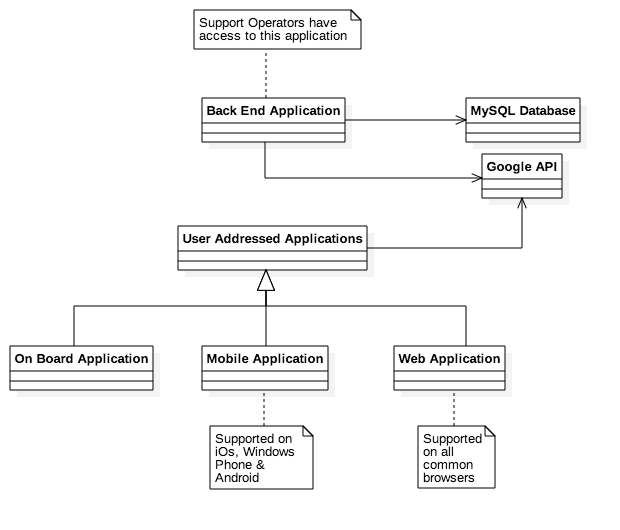
\includegraphics[width=0.9\textwidth ,height=0.9\textwidth ,center]{Images/SoftwareDistribution.png}
	 \end{center}
	 
	 
	 \subsection{Actors}
	  
	\begin{itemize}
 	 	\item \textit{Visitor}: a visitor is defined as a person who is not logged into the system. A visitor can see only the log-in page with a registration form and some common information ,such as the company's customer office contact information and terms of service.
  		\item \textit{Registered User}: is defined as any person using the system who is also logged into the system. A registered user can perform any of the above mentioned actions.
  		\item \textit{Car}: is defined as the vehicle to be used by a registered user. A car must be able to communicate to with the system all the time. If a car is available (i.e currently not reserved by a registered user) then its current location must be stored in the system so to be shown on all users' devices. As soon as the engine ignition starts , the car must time the vehicle's usage in order to charge the user the right amount of money. Once the user has parked the car inside a safe area and has exited, the car informs the system about the fee to charge ,locks the doors automatically and finally informs the system that it is available again.
  		\item \textit{Support operator}: The support operator is an employee who is trained and has a full grasp of the different software application .His job is to offer costumer support concerning software issues and help out in case of emergency.\\ Contrary to an user, he has access to the back-end software which enables him to overview the system status.
  		 
	\end{itemize}
	
	\subsection{User characteristics}
	There are no constraints about visitors : every person can access the main site and try to register.\\If a visitor wants to register there are some constraints to follow: 
	\begin{itemize}
		\item the user's has to be \textbf{at least 18} years old
		\item the user must have a \textbf{valid} driving license ( *aggiungere link al glossario *)
		\item the user must enter a valid payment method ( *aggiungere link al glossario *)
	\end{itemize}
	
	
	\subsection{Domain assumptions}
		\subsubsection{General Domain Assumptions}
			We hold the assumption that the system will be deployed in large metropolitan cities with a maximum of 3M inhabitants.\\
			We assume that the mean highest peak of activity is around dinner time on Fridays and Saturdays. We assume that during the peak the system will be used by around 50k people , 80\% of which gain access to the system through the Mobile Application, while the remaining 20\% through the Web Application.\\
			We assume that the the fleet of vehicles will be proportional to the number of inhabitants, reaching a peek of 300 vehicles in the biggest area.\\
		\subsubsection{User Assumptions}
		We assume that all users are provided with an enabled internet connection equipped with GPS tracking which is the only way to search, reserve and unlock a car.
		We assume that all active users carry their driving license with them and drive following the traffic code\footnote{\url {http://www.mit.gov.it/mit/site.php?p=normativa&o=vd&id=1&id_cat=&id_dett=0}}.
		\subsubsection{Vehicle Assumptions}
		* chiedere se e' bisogna inserire assunsiozioni sulla carica delle macchine etc...*		
			
	\subsection{Constraints}
	
	\subsubsection{Software Limitations}
	The Mobile and Web Application can not exceed 50MB of RAM usage.\\
	The On-Board application can not exceed 75MB of RAM usage.\\
	The Back-End application cannot exceed 100GB of RAM usage.
	\newpage
	\subsubsection{Hardware limitations}
	The Mobile Application must be available for the following mobile operating systems:
	\begin{itemize}
		\item iOS version 7.0 or higher.
		\item Android version 4.0 or higher.
		\item Windows Phone 8 or higher.
	\end{itemize}
	The applications must interface with Google Maps API \footnote{\url{https://developers.google.com/maps/documentation/javascript/}} and follow the design guidelines provided by each platform \footnote{\url{https://developer.android.com/design/index.html}} \footnote{\url{https://developer.apple.com/design/}}.\\
	\newline
	The Web Application must be developed in order to be correctly used by the following web browsers \footnote{\url{http://www.w3schools.com/browsers/default.asp}}:
		\begin{itemize}
		\item Mozilla Firefox
		\item Google Chrome
		\item Safari
		\item Microsoft Edge
		\item Opera
	\end{itemize}
	The on-board software system must be equipped with a GPS Module and interface Google Maps API. The following safety regulations must be followed:
	\begin{itemize}
		\item \textbf{Night mode}: an automatic night mode must be implemented. This will avoid that drivers get blinded by excessive brightness of the display.
		\item \textbf{Safe - area parking recognition}: the system must recognize whether the vehicle is parked in a safe-area or not.
		\item \textbf{Additional passenger recognition}: the system must recognize passenger. This feature is crucial for bonus credit distribution to the driver.
	\end{itemize}
	
	\subsubsection{Concurrency}
	The back-end application must be able to handle correctly multiple user requests without creating conflicts : if two users desire two reserve the same car simultaneously ,only one can be granted a reservation.
	
	\subsubsection{Regulatory Policies}
	\begin{itemize}
		\item \textbf{Privacy Policy}: Data should be collected and stored following the privacy policy guidelines provided by Mozilla Foundation \url{https://developer.mozilla.org/en-US/Marketplace/Publishing Policies_and_Guidelines/Privacy_policies}
		\item Network connections must be encrypted.
		\item Data storage on PowerEnjoy databases must be encrypted
	\end{itemize}
		

	\subsection{Functional Requirements}
	\textbf{1.Mobile and Web Application}
	\begin{itemize}
	 \item{\textbf{[R1.1]}}: Allow a guest to register entering all relevant personal data and a valid driving license whose validity will be check on the spot
	 \item{\textbf{[R1.2]}}: Allow a registered user to log-in
	 \item{\textbf{[R1.3]}}: Allow a registered user to update his personal information
	 \item{\textbf{[R1.4]}}: Allow a registered user to search for an available vehicle given his position within a selected distance
	 \item{\textbf{[R1.5]}}: Allow a registered user to search for an available vehicle given an input position within a selected distance
	  \item{\textbf{[R1.6]}}: Allow a registered user reserve a selected vehicle.
	 \item{\textbf{[R1.7]}}: Allow a registered user to check his payment history
	 \item{\textbf{[R1.8]}}: Allow a registered user to recover his account log-in information in a secure way
	 \item{\textbf{[R1.9]}}: Allow a registered user to search for an available vehicle given an input position.
	 \item{\textbf{[R1.10]}}: Allow a registered user to unlock \emph{his/her} reserved car if the user is nearby.
	 \item{\textbf{[R1.11]}}: **Chiedere per cancellazione prenotazioni**
	 	\end{itemize}

	\textbf{2.On-Board Application}
	\begin{itemize}
	 \item{\textbf{[R2.1]}}: Allow a registered user to correctly identify himself/herself by entering a user specific pin-code
 	 \item{\textbf{[R2.2]}}: Enable a registered user to keep track of the distance covered , time spent using the car ,the current owed fee and the remaining battery charge.
 	 \end{itemize}
 	 
 	 \textbf{3.Back-End Application}
	\begin{itemize}
	 \item{\textbf{[R3.1]}}: .
 	 \end{itemize}
	
	\subsection{Non functional Requirements -> qua o in paragrafo 3?} 
		Some non functional requirements have been to be necessary in the to be developed system in order to provider a correct operation flow and an optimized UX.
		\begin{itemize}
			\item \textit{User friendliness}: the Mobile/Web as well as the On-Board Application must be easily handled by the average web user with basic web knowledge.
			\item \textit{Performance}: to supply a suitable service the system must be responsive even at peak activity times. To achieve this client-server transaction must be reduced to a minimum.
		 	\item \textit{Reliability}: the PowerEnjoy service must be active 24h/24h . Maintenance must be performed without compromising functionality. At all the time , a user must be able to be charged the owed fee.	
		 	\item \textit{Data integrity and availability}: 
		 	Data have to be always available and accessible.Data availability can be achieved by duplicating data on back-up servers. For instance the use of RAID, mirroring and backup could present a valid solution.

		 	\item \textit{Maintainability}: the software should be implemented so as to be as modular as possible to allow future expansions and easy modifications.\\Google API are required but can be easily updated from time to time on all systems.
		 	\item \textit{Security}: user accounts are provided with two factor authentication with a code sent to the user's mobile phone to add a secure connection method to the system. Sensible user information are stored using a hashing mechanism .\\User data input should be filtered to avoid malicious modifications ( i.e SQL Injections). \\All connections should be encrypted and run on a secure HTTPS protocol with valid certificates that uses the secure TSL protocol to avoid Man in the Middle Attacks.
		\end{itemize}
		
	\subsection{Future implementation}
	The system must be as scalable as possible: future implementations can require a deployment in very large metropolitan cities that exceed by far the maximum amount of planned users.\\ An important thing to keep in mind is that the nature of vehicles could change in the distant future : not only cars , but also electric powered motorcycles could be added to the PowerEnjoy vehicle fleet.This means that the on-board software should be as expandable as possible using for instance Hierarchy Design Patterns in the vehicle type definition.
	 

\newpage
\FloatBarrier

\section{\Large Specific Requirements}
\subsection{External Interface Requirements}
 This section is dedicated to illustrate the mockups of the user interfaces.
 \FloatBarrier
 \subsubsection{Mobile Application}
 	
		\begin{figure}
		 \vspace{-17cm}	
		 \minipage{0.50\textwidth}
		 \centering	
		 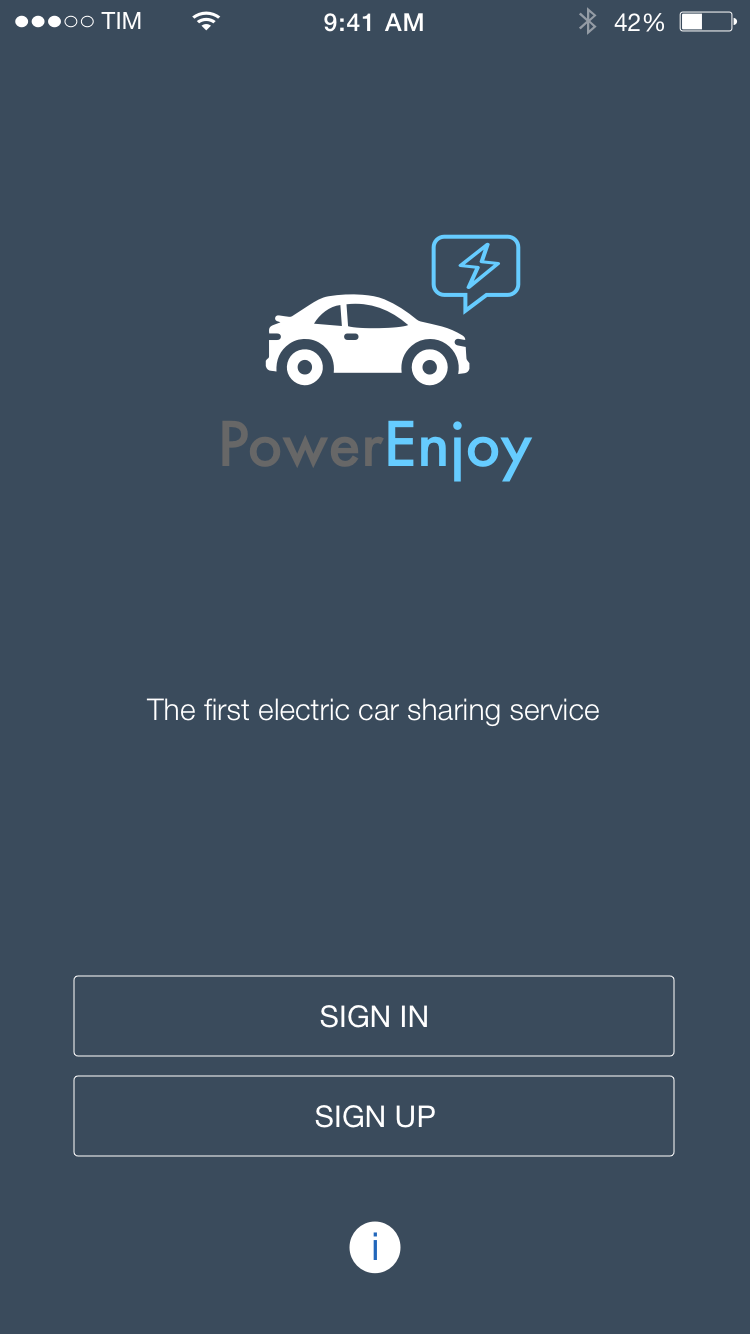
\includegraphics[scale=0.25]{Images/mobileApp/Home.png}
		 \caption{Home}
		 \endminipage
		 \minipage{0.50\textwidth}
		 \centering
 	 	  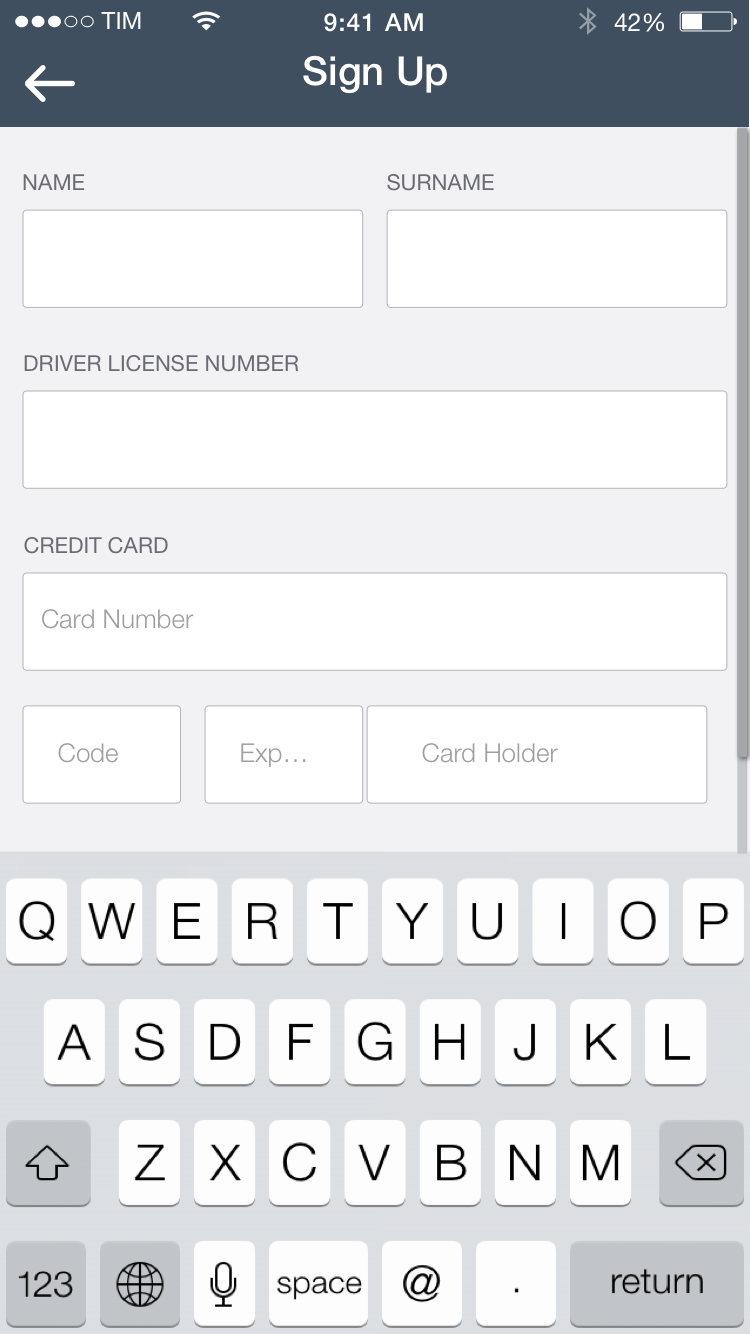
\includegraphics[scale=0.25]{Images/mobileApp/Register.png}
		  \caption{Sign Up}
		  \endminipage
 	 	\end{figure}
 	 	
 	 	\begin{figure}
		 \minipage{0.50\textwidth}
		 \centering	
		 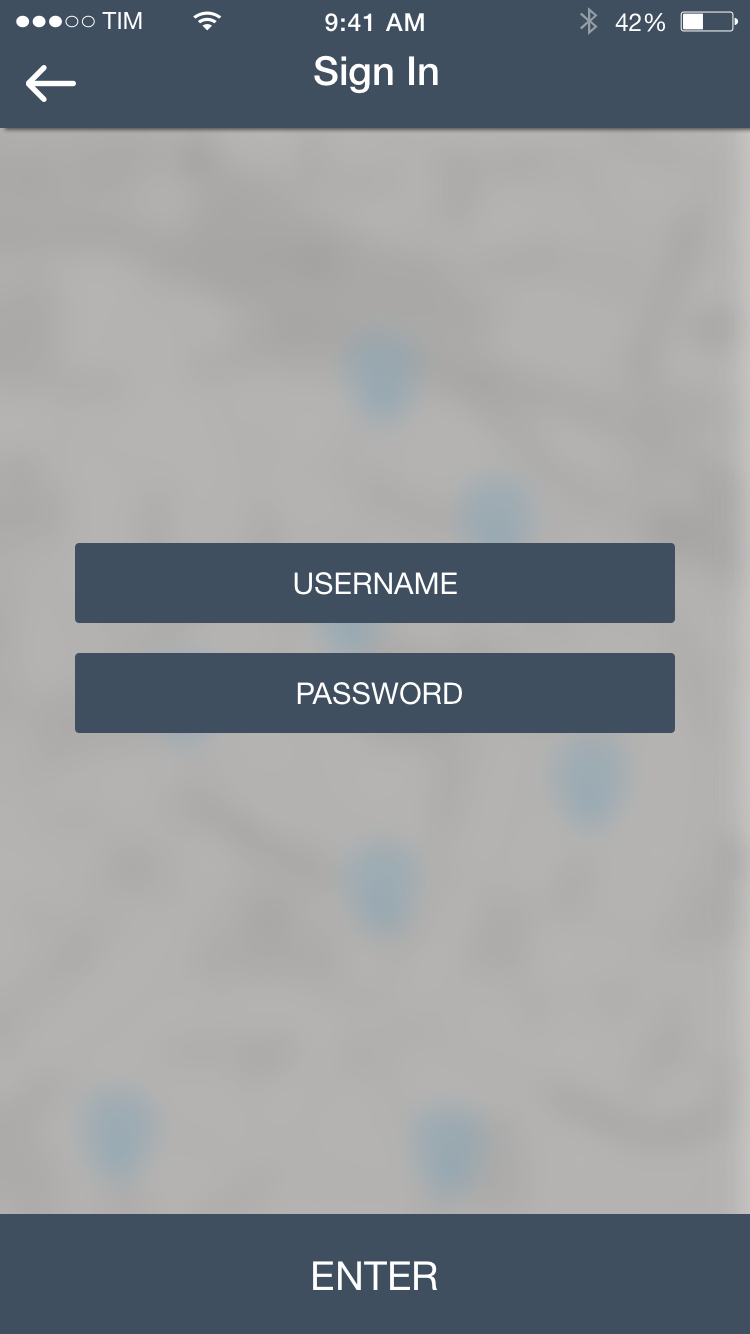
\includegraphics[scale=0.25]{Images/mobileApp/SignIn.png}
		 \caption{Sign In}
		 \endminipage
		 \minipage{0.50\textwidth}
		 \centering
 	 	  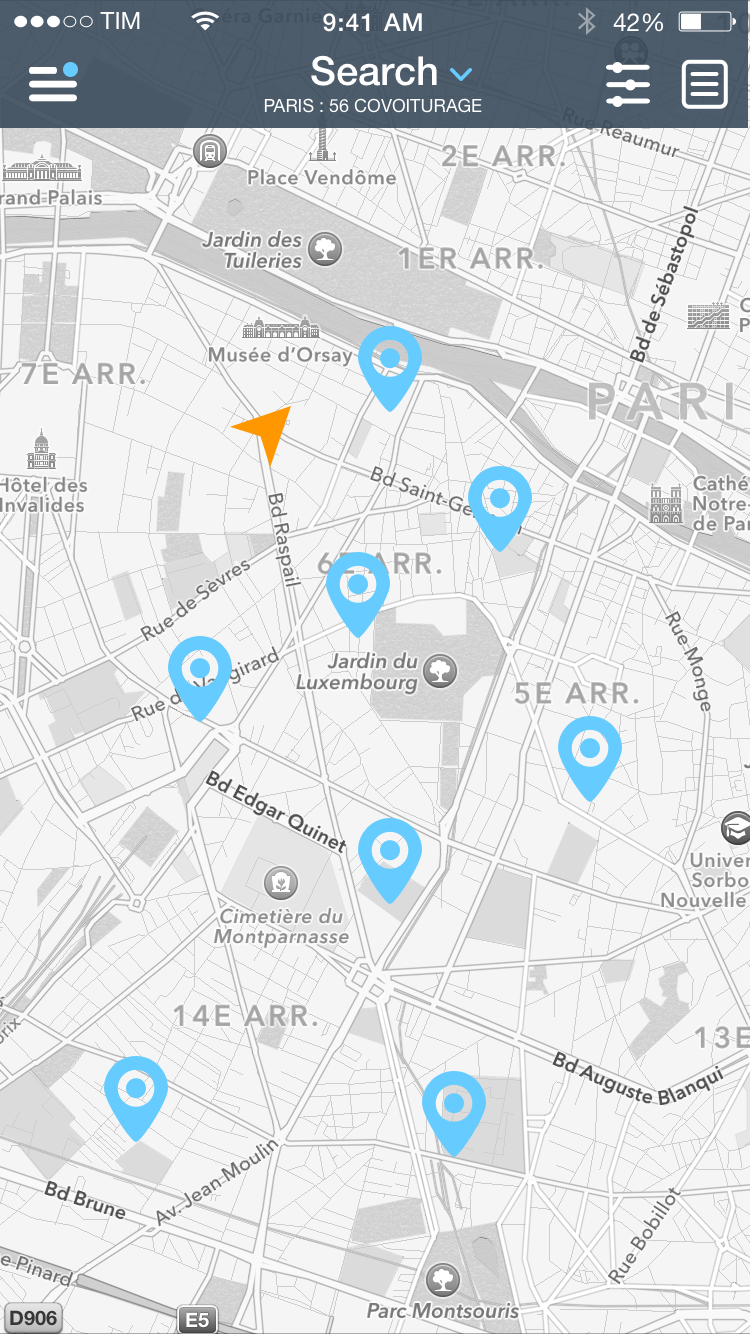
\includegraphics[scale=0.25]{Images/mobileApp/RicercaMappa.png}
		  \caption{Search}
		  \endminipage
 	 	\end{figure}

		\begin{figure}
		 \minipage{0.50\textwidth}
		 \centering	
		 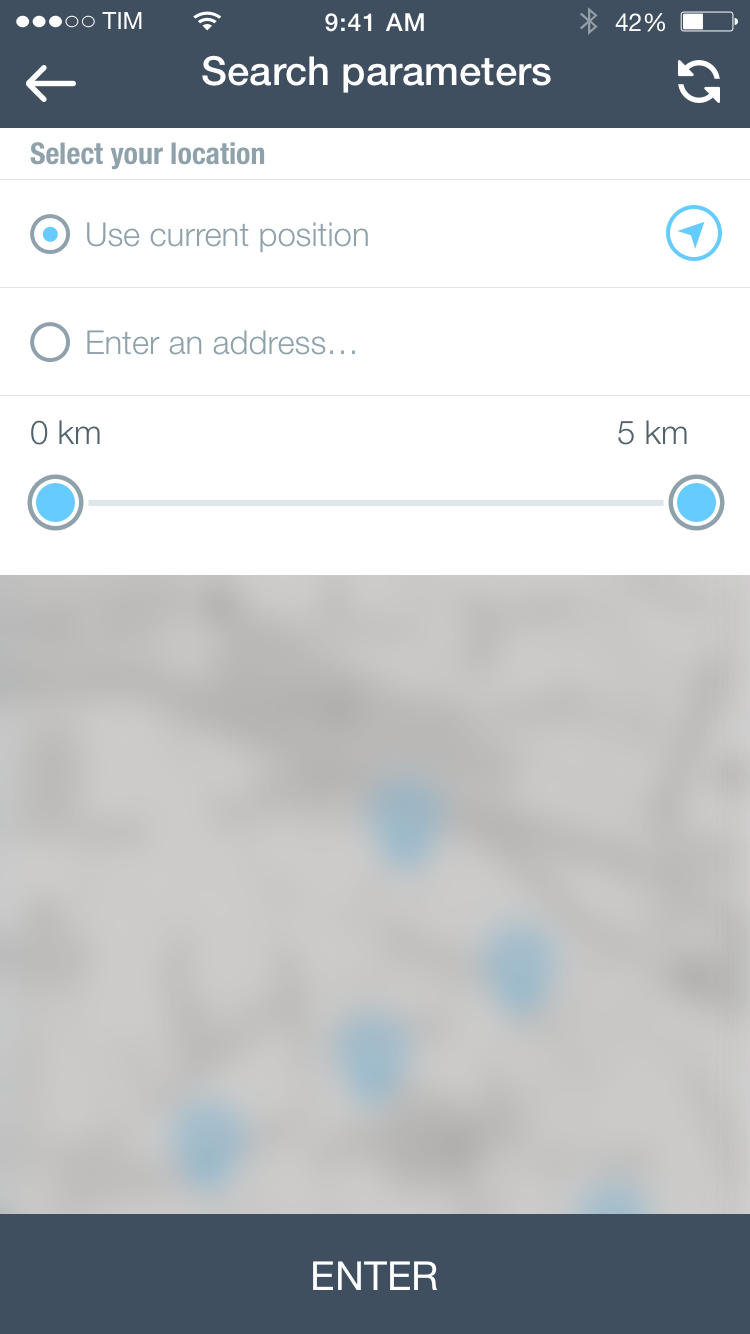
\includegraphics[scale=0.25]{Images/mobileApp/Param.png}
		 \caption{Address input}
		 \endminipage
		 \minipage{0.50\textwidth}
		 \centering
 	 	  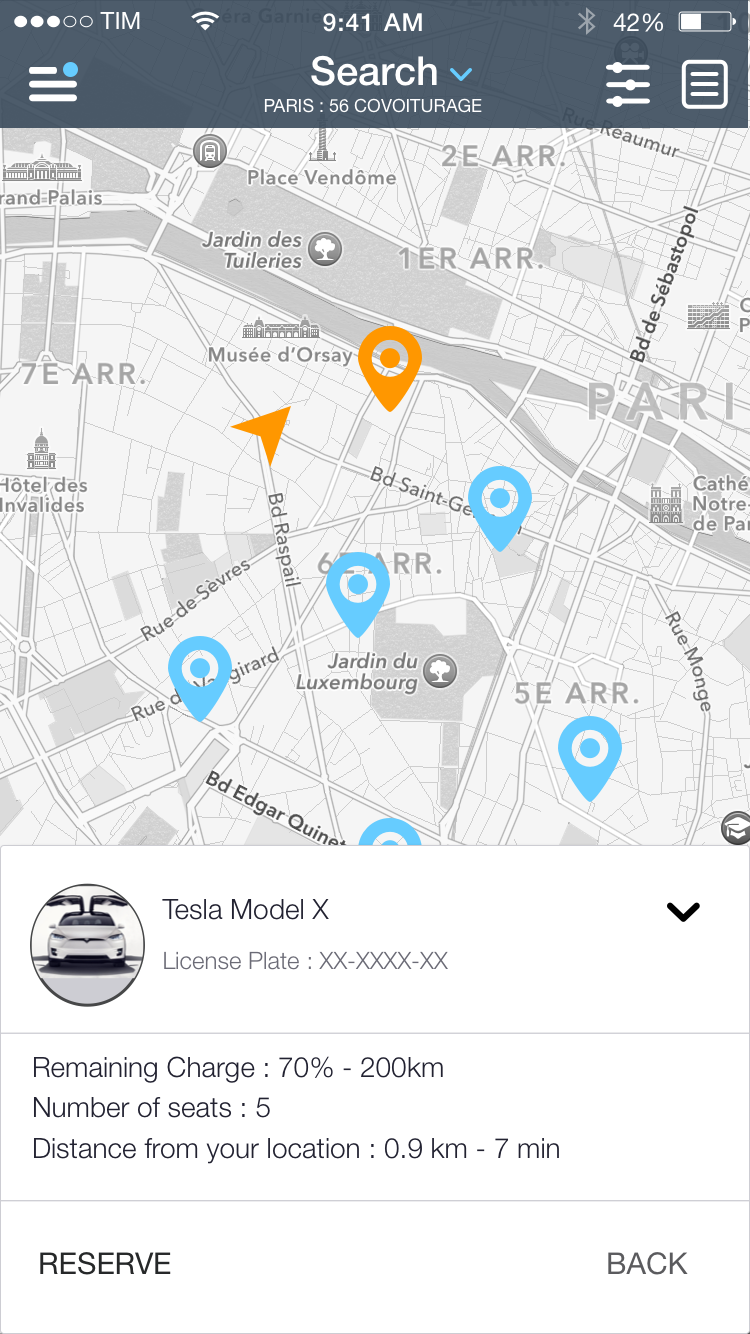
\includegraphics[scale=0.25]{Images/mobileApp/SelCar.png}
		  \caption{Car Selection}
		  \endminipage
 	 	\end{figure}
 	 	
 	 	\begin{figure}
		 \minipage{0.50\textwidth}
		 \centering	
		 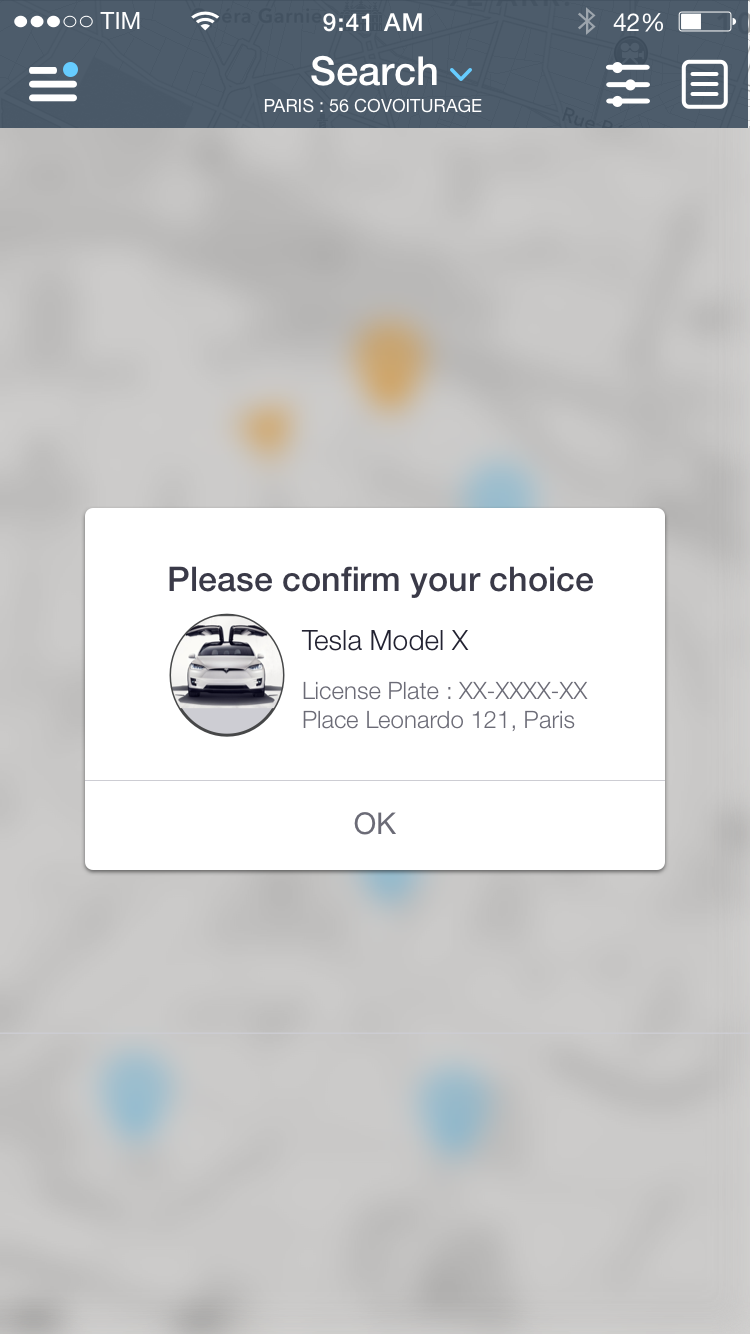
\includegraphics[scale=0.25]{Images/mobileApp/Conferma.png}
		 \caption{Confirm selection}
		 \endminipage
		 \minipage{0.50\textwidth}
		 \centering
 	 	  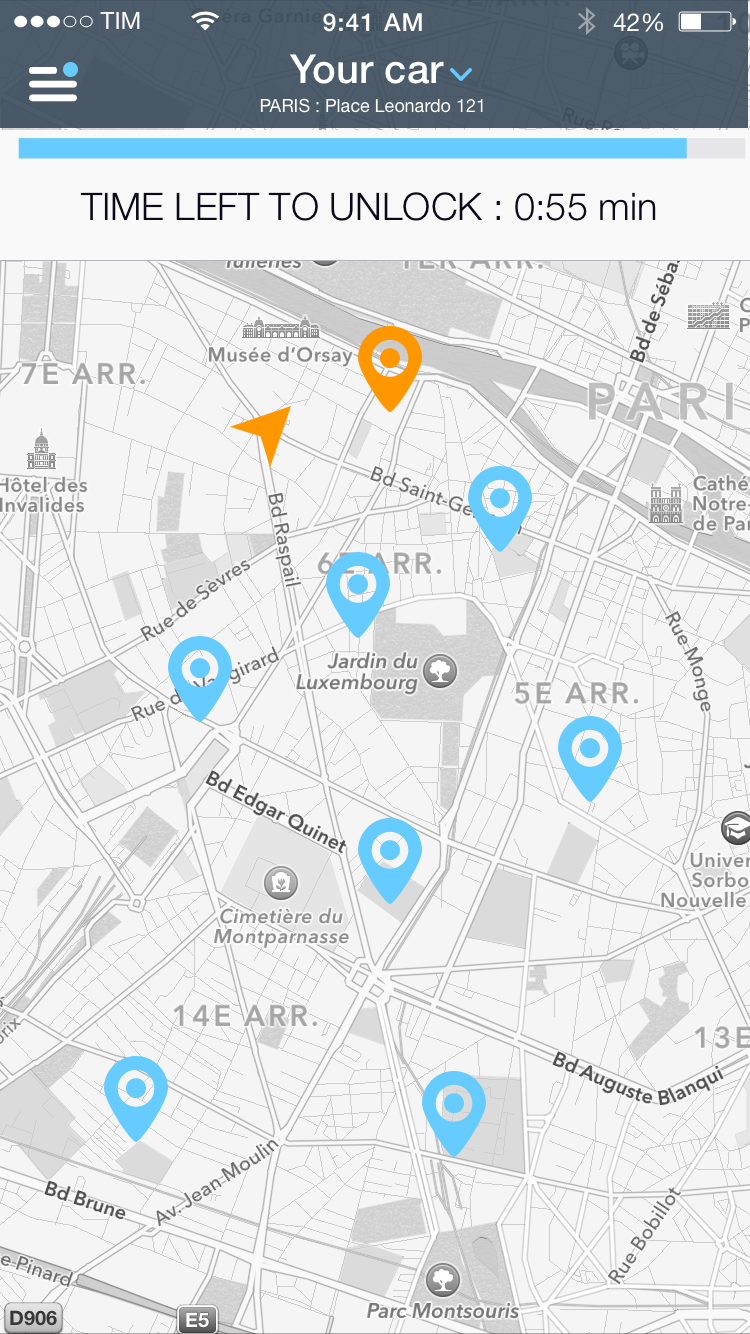
\includegraphics[scale=0.25]{Images/mobileApp/TimeLeft.png}
		  \caption{Time left to unlock}
		  \endminipage
 	 	\end{figure}
 	 	
 	 	\begin{figure}
		 \minipage{0.50\textwidth}
		 \centering	
		 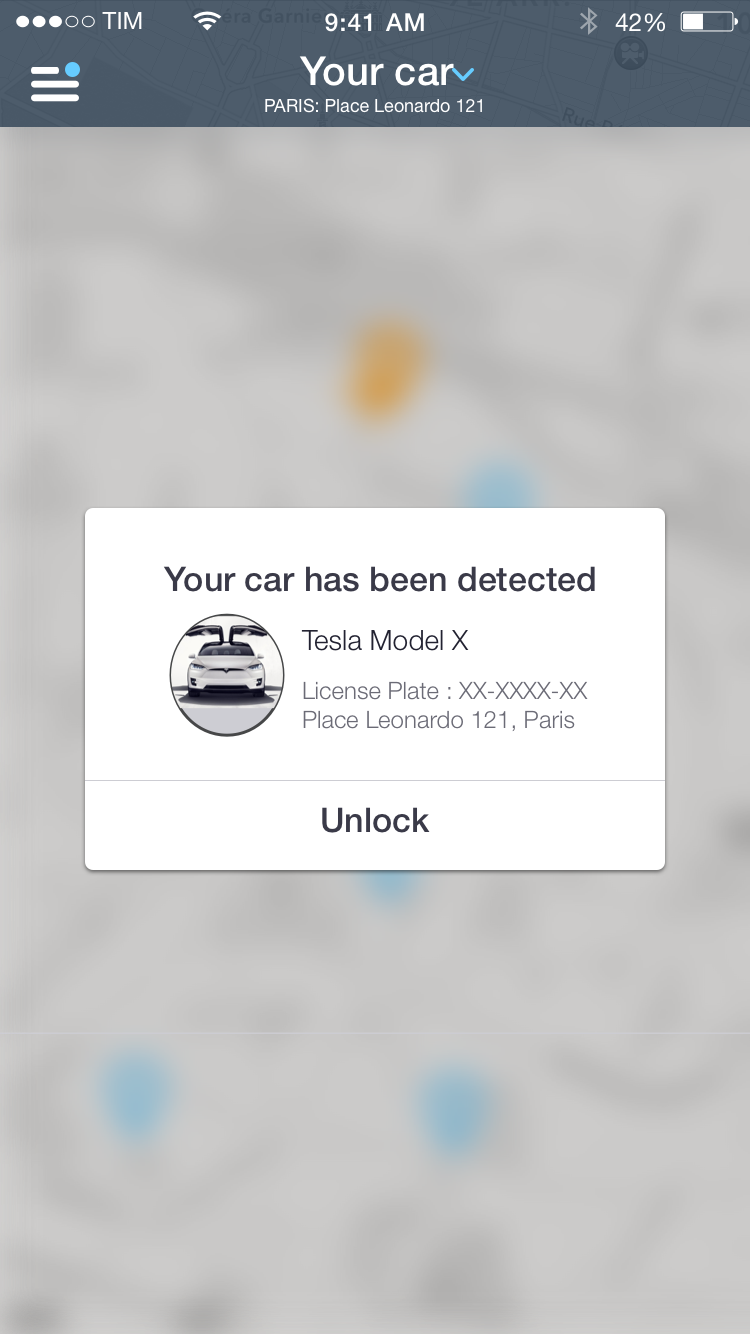
\includegraphics[scale=0.25]{Images/mobileApp/Sblocca.png}
		 \caption{Unlock car}
		 \endminipage
		 \minipage{0.50\textwidth}
		 \centering
 	 	  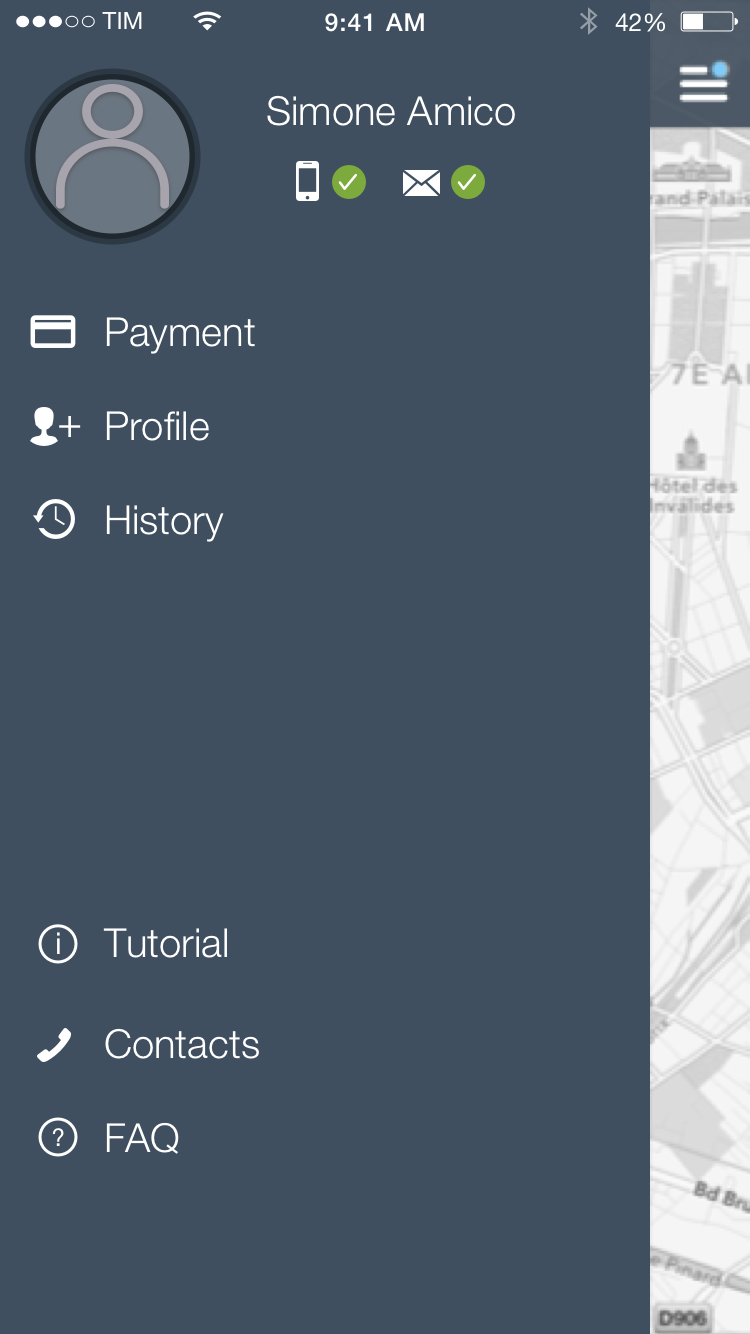
\includegraphics[scale=0.25]{Images/mobileApp/Menu.png}
		  \caption{Menu}
		  \endminipage
 	 	\end{figure}
 	 	
 	 \FloatBarrier
 	 \subsubsection{Web Application}
 	  	\begin{figure}
		\centering	
		\vspace{-14cm}		 
		 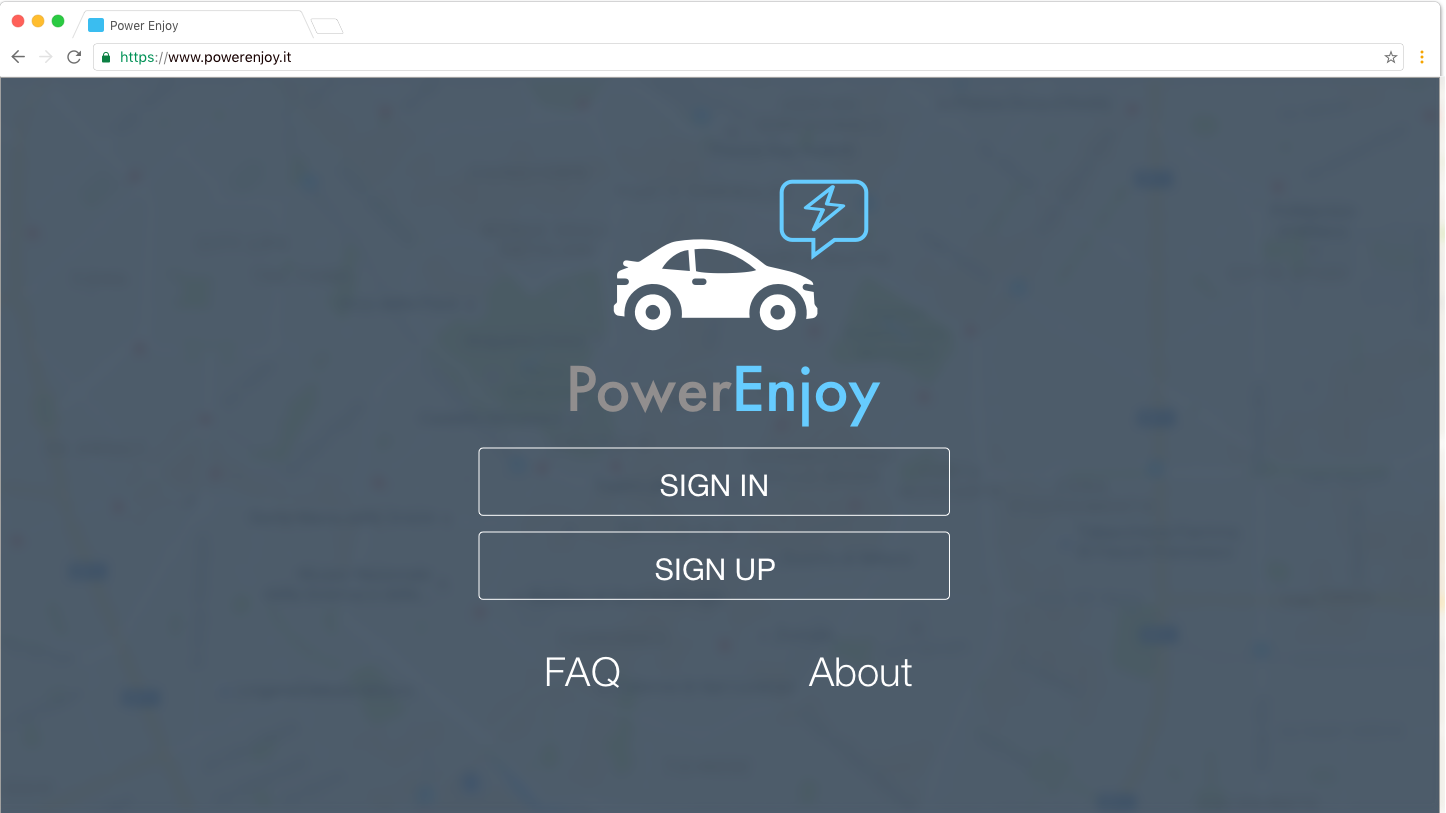
\includegraphics[scale=0.28]{Images/webApp/Homepage.png}
		 \caption{Homepage}
		 \centering
 	 	  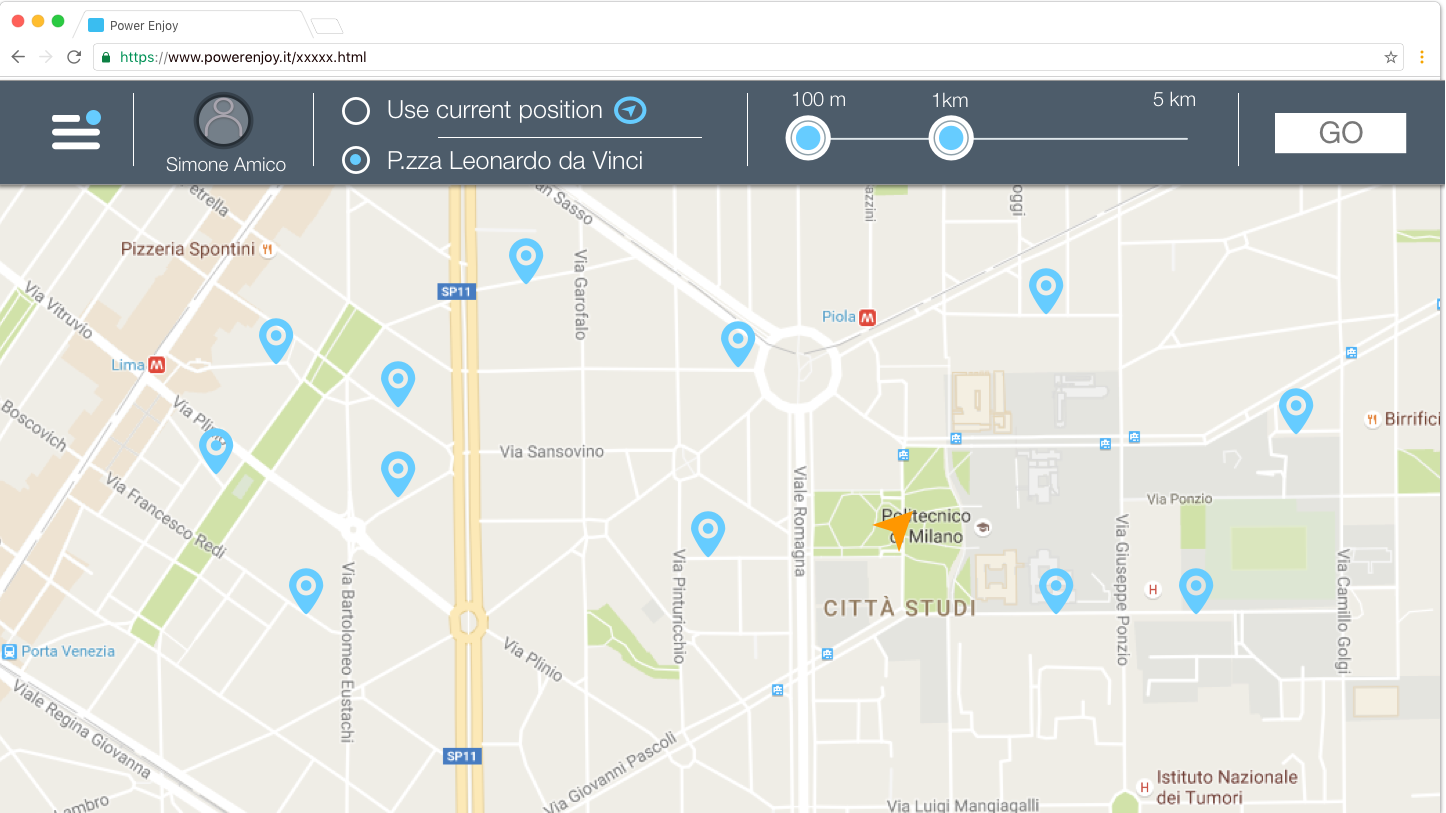
\includegraphics[scale=0.28]{Images/webApp/MainSearch.png}
		  \caption{Main page with map an car locations}
 	 	\end{figure}
 	 	
 	 	\begin{figure}
 	 	 \centering
 	 	 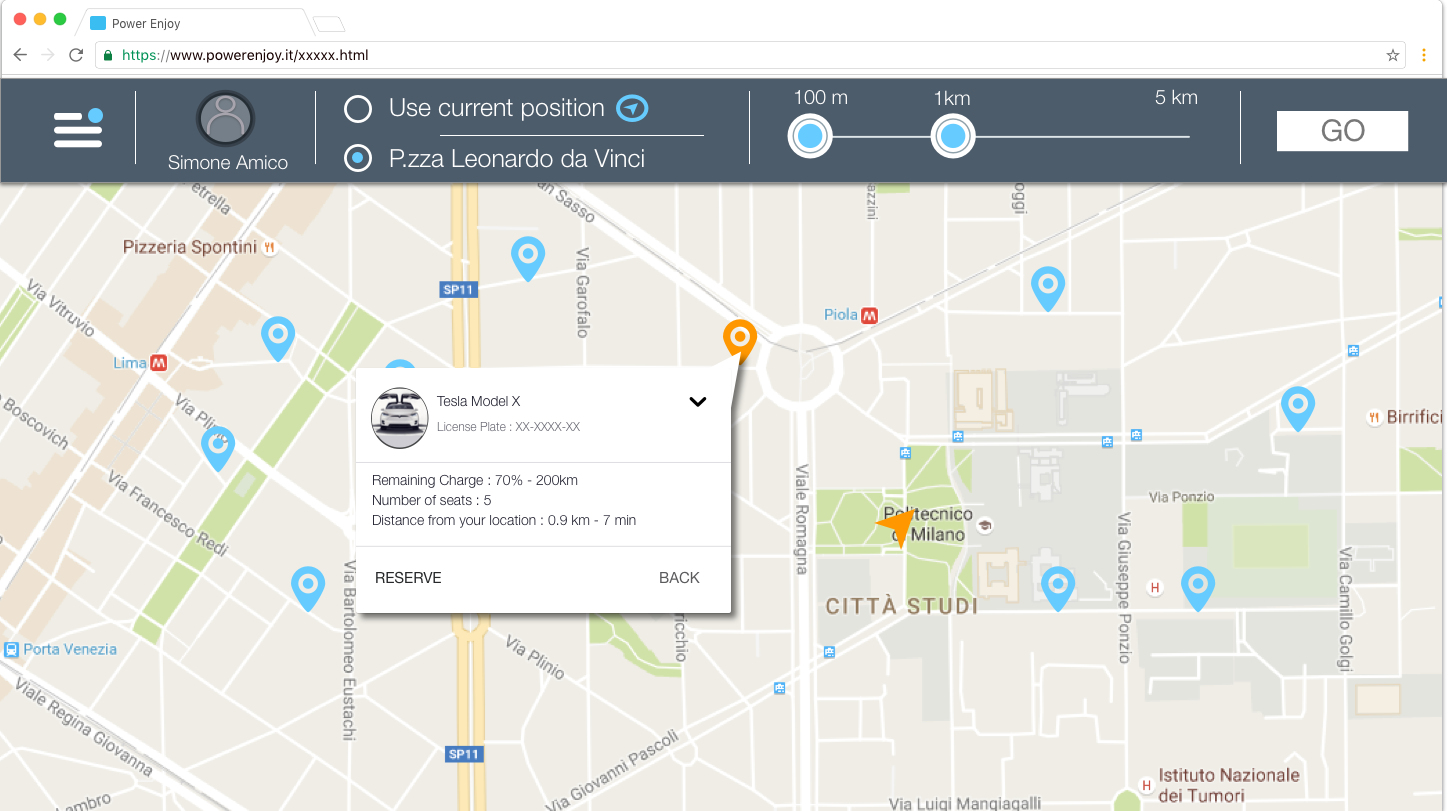
\includegraphics[scale=0.28]{Images/webApp/MainSearchCar.png}
		 \caption{Main page with car selection}
 	 	 \centering
 	 	 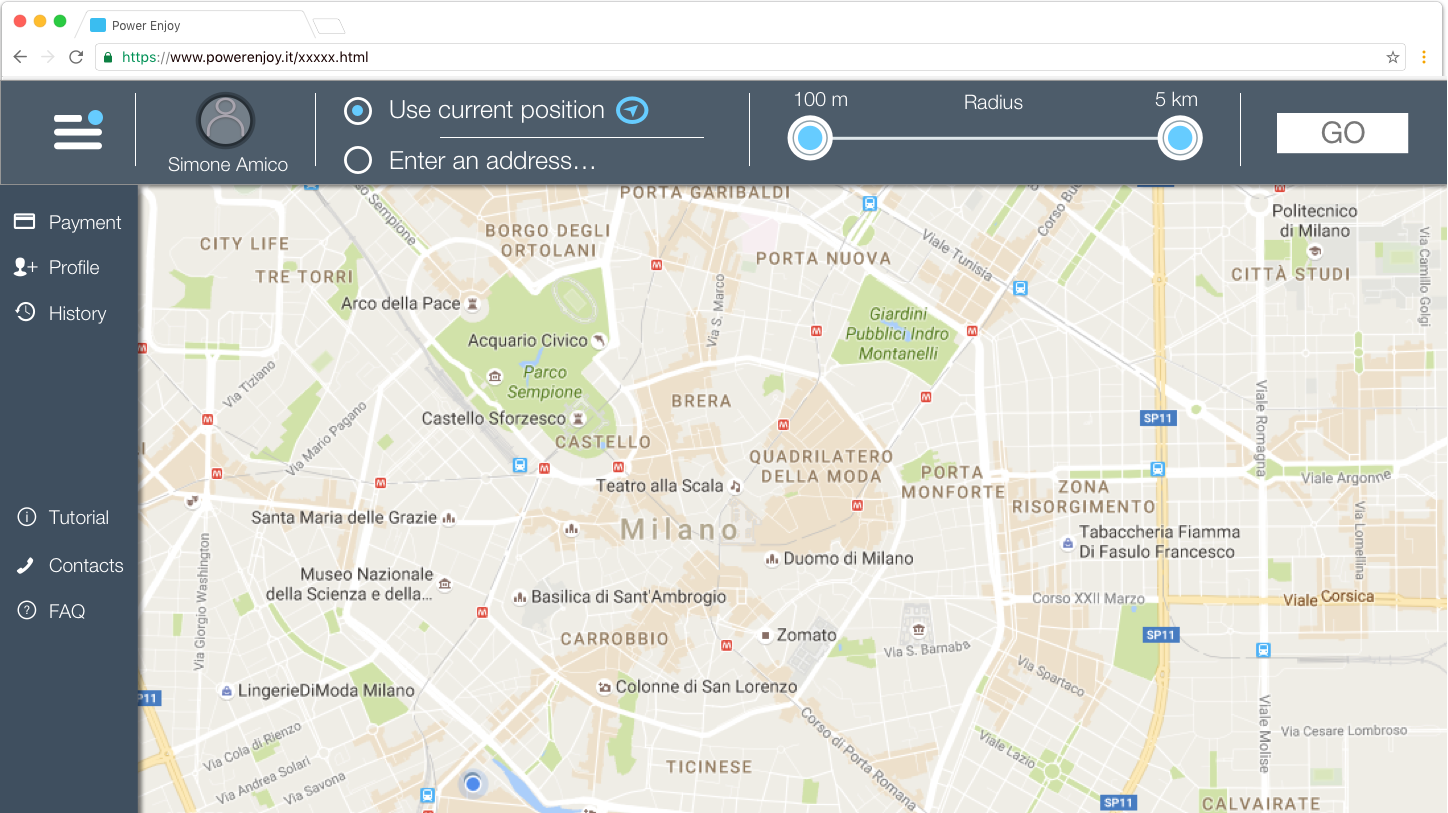
\includegraphics[scale=0.28]{Images/webApp/MainMenu.png}
		 \caption{Main page with account info bar}
		\end{figure}
		
	 \FloatBarrier
 	 \subsubsection{On-Board Application (Touch)}
 	 	 \begin{figure}
		 \centering	
		\vspace{-17cm}		 
		 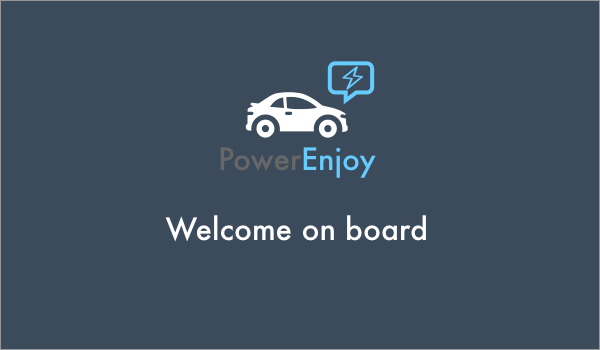
\includegraphics[scale=0.6]{Images/onBoard/Welcome.png}
		 \caption{Welcome screen}
		 \centering
 	 	  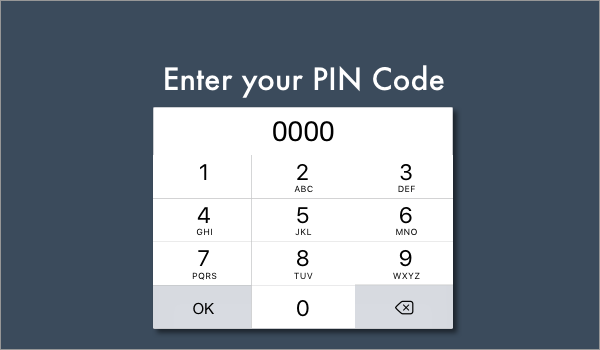
\includegraphics[scale=0.6]{Images/onBoard/Pin.png}
		  \caption{Pin request}
 	 	\end{figure}
 	 	 
 	 	\begin{figure}
		 \centering	
		 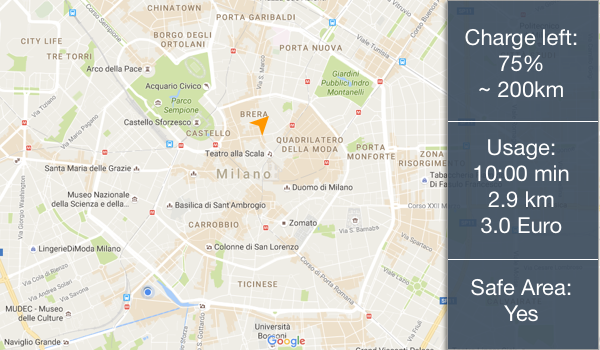
\includegraphics[scale=0.6]{Images/onBoard/Main.png}
		 \caption{Main screen}
 	 	\end{figure}
 	 	
 	   \FloatBarrier
 	 	\subsection{Scenarios}
 	
 	 	
 	 	
 	 

 	 	
		
	 	 

\end{document}